\chapter{Vastusten värikoodit}\label{varikoodit}
Arduinon mukana tulevissa vastuksissa on käytössä joko kahdenlaisia vastusmerkintöjä, joko neljällä tai viidellä viivalla.

Näistä viimeinen kertoo kuinka tarkasti vastuksen arvo osuu annettuun arvoon, ja nämä viivat ovat usien kultaisia tai hopeisia. Tämän avulla voit yrittää tunnistaa kummasta päästä vastuksen arvoa ollaan lukemassa. 

Kaksi tai kolme ensimmäistä viivaa kuvaa vastuksen numeroarvoa ja kolmas tai neljäs viiva kuvaa vastuksen kokoluokkaa (eli kerrointa, esimerkiksi $k=1000$). 

%%%%%%%%%%%%%%%%%%%%%%%%%%%%%%%%
\definecolor{rbrown}{HTML}{996633}
\definecolor{rred}{HTML}{FF0000}
\definecolor{rorange}{HTML}{FF9900}
\definecolor{ryellow}{HTML}{FFFF00}
\definecolor{rgreen}{HTML}{228b22}
\definecolor{rblue}{HTML}{0047AB}
\definecolor{rviolet}{HTML}{800080}
\definecolor{rgrey}{HTML}{CCCCCC}
\definecolor{rwhite}{HTML}{FFFFFF}
\definecolor{kulta}{HTML}{FFD700}
\definecolor{hopea}{HTML}{C0C0C0}
%%%%%%%%%%%%%%%%%%%%%%%%%%%%%%%
\begin{minipage}{0.4\textwidth}
Kahden tai kolmen ensimmäisen viivan värit ja niitä vastaavat numerot:

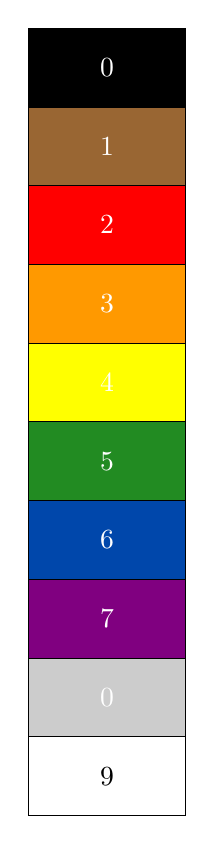
\begin{tikzpicture}
  \draw[fill=black] (0,0) rectangle ++(2,1) node[pos=(0.5),white] {0};
  \draw[fill=rbrown] (0,-1) rectangle ++(2,1) node[pos=0.5,white] {1};
    \draw[fill=rred] (0,-2) rectangle ++(2,1) node[pos=(0.5),white] {2};
  \draw[fill=rorange] (0,-3) rectangle ++(2,1) node[pos=0.5,white] {3};
    \draw[fill=ryellow] (0,-4) rectangle ++(2,1) node[pos=(0.5),white] {4};
  \draw[fill=rgreen] (0,-5) rectangle ++(2,1) node[pos=0.5,white] {5};
    \draw[fill=rblue] (0,-6) rectangle ++(2,1) node[pos=(0.5),white] {6};
  \draw[fill=rviolet] (0,-7) rectangle ++(2,1) node[pos=0.5,white] {7};
  \draw[fill=rgrey] (0,-8) rectangle ++(2,1) node[pos=(0.5),white] {0};
  \draw[fill=rwhite] (0,-9) rectangle ++(2,1) node[pos=0.5,black] {9};
  %\draw[draw=black] (11.1,5.5) rectangle ++(0.3,0.3);
\end{tikzpicture}
\end{minipage}
\begin{minipage}{0.3\textwidth}
Kertoimen suuruus, $10^{x}$, missä $x$ on listassa annettu luku:

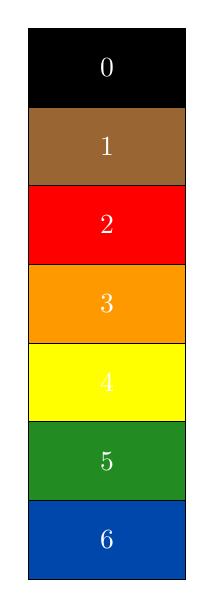
\begin{tikzpicture}
  \draw[fill=black] (0,0) rectangle ++(2,1) node[pos=(0.5),white] {0};
  \draw[fill=rbrown] (0,-1) rectangle ++(2,1) node[pos=0.5,white] {1};
    \draw[fill=rred] (0,-2) rectangle ++(2,1) node[pos=(0.5),white] {2};
  \draw[fill=rorange] (0,-3) rectangle ++(2,1) node[pos=0.5,white] {3};
    \draw[fill=ryellow] (0,-4) rectangle ++(2,1) node[pos=(0.5),white] {4};
  \draw[fill=rgreen] (0,-5) rectangle ++(2,1) node[pos=0.5,white] {5};
    \draw[fill=rblue] (0,-6) rectangle ++(2,1) node[pos=(0.5),white] {6};
\end{tikzpicture}
\end{minipage}
\begin{minipage}{0.2\textwidth}
Toleranssin\\ suuruus:

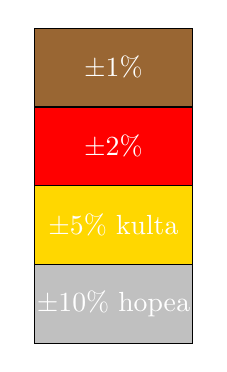
\begin{tikzpicture}
  \draw[fill=rbrown] (0,-1) rectangle ++(2,1) node[pos=0.5,white] {$\pm1\%$};
    \draw[fill=rred] (0,-2) rectangle ++(2,1) node[pos=(0.5),white] {$\pm2\%$};
  \draw[fill=kulta] (0,-3) rectangle ++(2,1) node[pos=0.5,white] {$\pm5\%$ kulta};
    \draw[fill=hopea] (0,-4) rectangle ++(2,1) node[pos=(0.5),white] {$\pm10\%$ hopea};
\end{tikzpicture}
\end{minipage}


\begin{table}[!h]
\caption {Paketissa mukana olevat vastukset.} \label{tab:varikooditv} 
\begin{center}
\begin{tabular}{c|c}
    Vastus & Kuvat  \\\hline\\
   $220\Omega$  & \includegraphics[width=0.5\textwidth]{kuvat/220.pdf} \\\hline\\
   $560\Omega$  & \includegraphics[width=0.5\textwidth]{kuvat/560.pdf} \\\hline\\
   $1\text{k}\Omega$  & \includegraphics[width=0.5\textwidth]{kuvat/1k.pdf} \\\hline\\
   $4.7\text{k}\Omega$  & \includegraphics[width=0.5\textwidth]{kuvat/4k7.pdf} \\\hline\\
   $10\text{k}\Omega$  & \includegraphics[width=0.5\textwidth]{kuvat/10k.pdf} \\\hline\\
$1\text{M}\Omega$  & \includegraphics[width=0.5\textwidth]{kuvat/1M.pdf} \\\hline\\
   $10\text{M}\Omega$  & \includegraphics[width=0.5\textwidth]{kuvat/10M.pdf} \\\hline
\end{tabular}
\end{center}
\end{table}

\begin{tcolorbox}[colback=red!10,colbacktitle=red,title=HUOM!]
Jos käytössäsi on yleismittari, voit tarkistaa vastuksen arvon sillä!
\end{tcolorbox}
